\documentclass[11pt]{article}
\usepackage{fullpage,url}
\usepackage{amsmath}
\usepackage{graphicx}

\usepackage[letterpaper,top=1in,bottom=1in,left=1in,right=1in,nohead]{geometry}
\usepackage{amsthm}

\setlength{\parindent}{0in}
\setlength{\parskip}{6pt}

\DeclareMathOperator{\E}{E}
\DeclareMathOperator{\Var}{Var}
\DeclareMathOperator{\Unif}{Unif}

\begin{document}
\thispagestyle{empty}
{\large{\bf Notes \hfill Danny Perry}}\\

{\LARGE{\bf Maximum Principle Proof by Fritz John}}
\vspace{0.2\baselineskip}
\hrule

Notes of proof of maximum principle for a parabolic PDE, from: F. John. "Partial Differential Equations".  New York: Springer-Verlag. 1982. pp. 215-216.


Let $\omega$ denote an open bounded set of $\Re^n$.  For a fixed $T>0$ we form the cylinder $\Omega$ in $\Re^{n+1}$ with base $\omega$ and height $T$:
\begin{align}
\Omega = \{(x,t)|x \in \omega, 0 < t < T \}
\end{align}
The boundary $\partial \Omega$ consists of two dijoint portions, a "lower" boundar $\partial'\Omega$, and an "upper" one $partial''\Omega$ (see Figure\ref{fig:drawing}):
\begin{align}
\partial'\Omega = \{(x,t)|eigher x \in \partial \omega, 0 \le t \le T or x \in \omega, t=0\} \\
\partial''\Omega = \{(x,t)|x \in \omega, t=T\}.
\end{align}
As in the second-order elliptic case the maximum of a solution of the heat equation in $\Omega$ is taken on $\partial \Omega$; but a more subtle distinction between the forwards and backwards t-directions makes itself felt:

\newtheorem{maxthrm}{Theorem}
\begin{maxthrm}
Let $u$ be continuous in $\bar{\Omega}$ and $u_t,u_{x_ix_k}$ exist and be continuous in $\Omega$ and satisfy $u_t-\triangle u \le 0$. Then
\begin{align}
\max_{\bar{\Omega}} u = \max_{\partial ' \Omega} u \label{eqn:thrm}
\end{align}
\end{maxthrm}

\begin{proof}
Let at first $u_t-\triangle u < 0$ in $\Omega$.  Let $\Omega_{\epsilon}$ for $0<\epsilon<T$ denote the set
\begin{align*}
\Omega_{\epsilon} = \{(x,t)|x\in \omega, 0<t<T-\epsilon\}.
\end{align*}
Since $u \in C^0(\bar{\Omega}_{\epsilon})$ there exists a point $(x,t) \in \bar{\Omega}_{\epsilon}$ with
\begin{align*}
u(x,t) = \max_{ \bar{\Omega}_{\epsilon} } u.
\end{align*}
If here $(x,t) \in \Omega_{\epsilon}$ the necessary relations $u_t = 0, \triangle \le 0$ would contradict $u_t - \triangle u < 0$.  If $(x,t) \in \partial '' \Omega_{\epsilon}$ we would have
\begin{align*}
u_t \ge 0, \triangle u \le 0
\end{align*}
leading to the same contradiction.  Thus $(x,t) \in \partial ' \Omega_{\epsilon}$, and
\begin{align*}
\max_{ \bar{\Omega}_{\epsilon} } u = \max_{ \partial ' \Omega_{\epsilon} } u \le \max_{ \partial ' \Omega } u.
\end{align*}
Since every point of $\bar{\Omega}$ with $t<T$ belongs to some $\bar{\Omega}_{\epsilon}$ and $u$ is continuous in $\bar{\Omega}$, (\ref{eqn:thrm}) follows. Let next $u_t - \triangle u \le 0$ in $\Omega$. Introduce
\begin{align*}
v(x,t) = u(x,t) - kt
\end{align*}
with a constant positive $k$.  Then $v_t-\triangle v = u_t-\triangle u - k < 0$ and
\begin{align*}
\max_{\bar{\Omega}} u = max_{ \bar{\Omega} } (v+kt) \le \max_{\bar{\Omega}} v + kT = \max_{\partial ' \Omega} v + kT \le \max_{\partial ' \Omega} u + kT.
\end{align*}

For $k \rightarrow 0$ we obtain (\ref{eqn:thrm}).


\end{proof}

\begin{center}
\begin{figure}
\centering
%\includegraphics[width=0.5\textwidth,angle=270]{scatter}
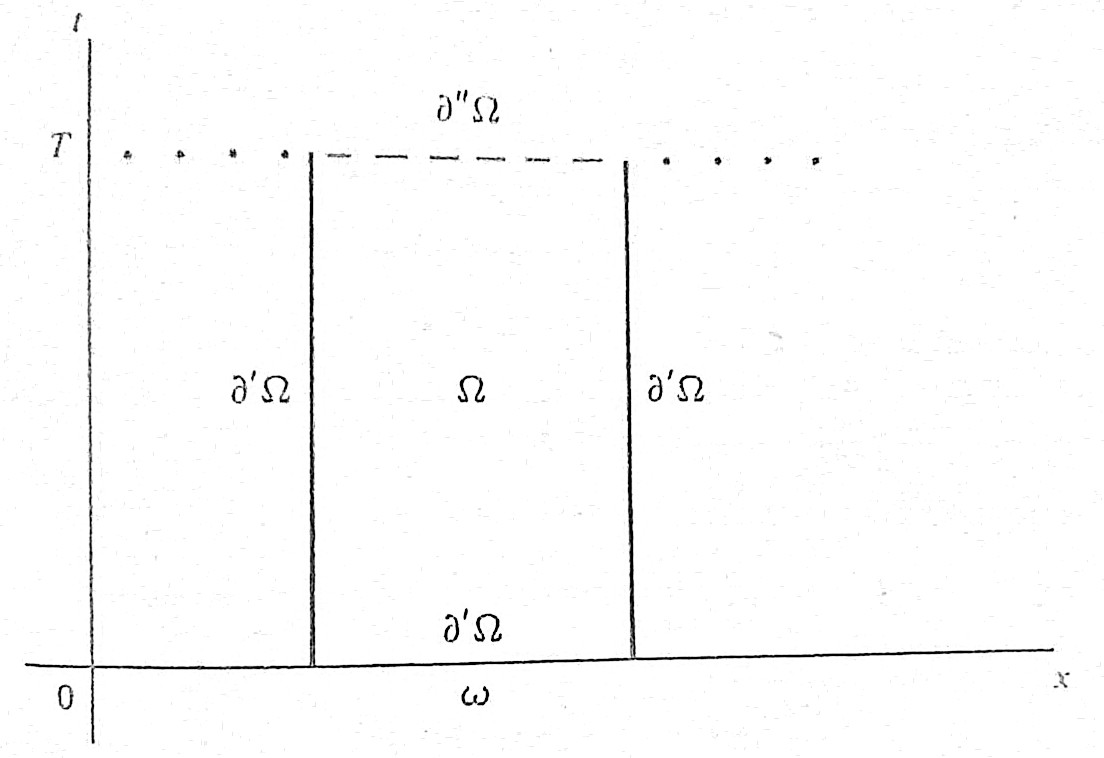
\includegraphics[width=0.5\textwidth]{drawing}
\caption{Illustration of the proof space, from book.}
\label{fig:drawing}
\end{figure}
\end{center}


\end{document}
